%======================= MINIATURIZE CNN FOR EMBEDDING ===========================
% TODO check figure captions
\graphicspath{{img/parking/}}

\chapter{Miniaturization of \acrlongpl{cnn} for Embedded Devices}
\label{ch:miniaturization}

One of the most significant limitations of \glspl{cnn} is that they often rely on computationally expensive deep models, which are slow for many applications including image classification.
Due to this limitation, methods based on efficient hand-crafted local features --- such as \acrshort{surf}, \acrshort{orb}, \acrshort{lbp}, etc.\ --- are predominantly adopted in vision systems where a computational power of a full-featured server is not available, e.g., mobile phones or embedded devices.

In this chapter, we explore the adoption and the miniaturization of \glspl{cnn} for efficient image classification.
We focused our investigation on reducing and evaluating deep models for embedded vision systems, i.e., smart cameras.
A smart camera is an embedded camera equipped with a limited computational and communication capabilities that can be used to process, extract, and send information contained in the captured images on board of the device itself.
Empowering smart cameras with the generalization and robustness of \glspl{cnn} for computer vision application represents one the most promising steps towards the evolution of smart environments~\cite{valera2005intelligent}.
Their ``smart'' nature makes them suitable for automated intelligent systems able to generate event descriptions and make decisions~\cite{belbachir2010smart}, thus making them attractive to a broad range of applications.

In our study, we focused on a specific application that is the visual occupancy detection of outdoor car parking lots in a decentralized fashion with smart cameras.
The motivation for the choice of this specific problem is manifold.
\begin{itemize}
    % easy problem formulation as 2-way classification
    % lack of deep learning solutions for the problem
    \item The problem of visual occupancy detection of parking spaces can be readily formulated as a binary image classification problem;
    this enabled us to focus on the engineering aspects of model reduction and its evaluation;
    moreover, state-of-the-art approaches tackling this problem are based on handcrafted features and shallow machine learning, while a deep learning solution could bring (and brought) to an improvement of the detection accuracy and robustness.

    % current systems vision solutions are centralized, with BW costs
    \item Parking lot occupancy detection systems are commonly implemented employing expensive magnetic ground sensors, while vision-based systems provide a more cost-effective solution;
    in our setup, a single smart camera can simultaneously monitor up to 50 parking slots at a cost significantly lower than the one required to install and maintain ground sensors for every slot.

    % decentralize for flexibility and bw cost
    \item In centralized solutions, ``dumb'' cameras send their video feeds to a server which processes them;
    a decentralized solution instead brings a reduction of the communication overhead and the elimination of the computing bottleneck, thus increasing even further the scalability of the solution;
    moreover, an intelligent infrastructure provides flexibility in its application, e.g., the same cameras could be used for perimeter surveillance during night hours.

\end{itemize}
%
While visual approaches to parking lot occupancy detection are not new~\cite{dan2002parking,wu2007robust,del2015vacant,de2015pklot}, the usage of solely visual information still poses challenges in terms of robustness.
Numerous solutions are tailored to specific scenarios and hardly generalize well to different ones, such as a different parking lot, viewpoint, light conditions, or occlusion patterns.

In our investigation, we proposed a decentralized and efficient vision system based on smart cameras and \gls{dl} for parking lot occupancy detection.
We presented a reduced \gls{cnn} suitable for embedded devices with which we implement the classification logic under the occupancy detection task.
We applied a robust experimental protocol on publicly available datasets to compare the proposed approach to the state-of-the-art methods and deep models and assess its generalization properties.
Despite being evaluated on a specific application, the solution we adopted is general and can be easily transferred to other vision-based tasks.
In addition, we contributed with a publicly available dataset of the parking lot images captured by multiple cameras called \emph{CNRPark-EXT} that enabled us to thoroughly test the robustness of our solution to multiple sources of errors.

The chapter is organized as follows.
In \ref{sec:mini:related-work}, we introduce the work related to parking lot occupancy detection, focusing on vision-based solutions more related to our proposal.
In \ref{sec:mini:occupancy-detection}, we propose and describe the \gls{cnn} model specifically designed to be executed on smart cameras which implements the parking slot classification pipeline.
In \ref{sec:mini:datasets}, we present the already available and newly collected datasets used to evaluate and compare our approach.
\ref{sec:mini:evaluation} presents the proposed experimental setup to compare our approach to the state of the art and evaluate its robustness to multiple aspects.
\ref{sec:mini:deployment} briefly describes the deployment of our solution in a real scenario and gives an overview of the overall system.

The research presented in this chapter was published in~\cite{amato2016car,amato2017deep}, and the provided resources --- e.g., datasets and trained models --- are available at \url{http://cnrpark.it}.

\section{Visual Occupancy Detection and Related Work}
\label{sec:mini:related-work}

Techniques for car parking occupancy detection are of great importance for the effective management of car parking lots.
Knowing in real-time the availability of free parking spaces and communicating it to the users can be of great help in reducing the queues, traffic jams, and the time required to find an available parking slot.
In the following paragraphs, we review some of the work targeting this problem, focusing on vision-based methods.

\paragraph{\gls{ml}-based approaches}
% Occupancy Detection w/o CNNs
Many attempts before the \gls{dl} era were implemented by classical \gls{ml} methods applied on handcrafted visual features.
\citet{dan2002parking}, one of earliest work using this approach on the subject, used \glspl{svm} on color features to classify regions of the parking lot as `car` or `empty-space`.
Among the challenges arose by the task, the problem of occlusions due to obstacles or camera angle is one of the most significant.
\citet{wu2007robust} tried to overcome occlusion by neighboring cars by also considering the neighbor parking slots of the one to be classified.
The \gls{svm} classifier for a slot is defined over the color features computed across three slots (the slot itself and the two neighbor slots).
\citet{tsai2007vehicle} used multiple handcrafted features and a Bayesian classifier to deal with the problem of light changes, while
\citet{huang2013vacant} employed a Bayesian hierarchical framework based on a 3D model of the parking spaces.
Similarly, \citet{delibaltov2013parking} proposed a method based on a 3D model of every parking slot in order to account for occlusions when classifying a slot as vacant or occupied.
In~\cite{jermsurawong2014one}, a feed-forward neural network defined on multiple handcrafted visual features is used to model the occupancy status of slots and the parking demand.
% they present robust results for night and day classifiers in a one-day long evaluation based on 126 parking spaces.
In~\cite{de2015pklot}, the authors employed ensembles of \gls{svm} classifiers based on multiple textural features --- such as \gls{lbp}, \gls{lpq}, and their variations --- and they present a dataset of roughly 700,000 images of parking spaces coming from three different cameras used in their experiment.
\citet{del2015vacant} proposed a temporal analysis of the video frames based on background subtraction to detect and track parking and leaving vehicles.
Similarly, \citet{masmoudi2014} propose to overcome the occlusion problem by visually tracking cars entering or leaving a parking space.

\paragraph{Non-vision approaches}
In addition to approaches using visual techniques and commercial solutions using ground sensors, there are techniques harnessing sensors installed on cars or carried by the drivers.
In~\cite{caicedo2012prediction}, the authors argue that occupancy detection can be solved by interacting with smart in-vehicle navigation systems.
\citet{lan2014intelligent} instead proposed to harness sensors in smartphones and other devices to collect real-time parking availability information.
%
\paragraph{\gls{dl}-based approaches}
To the best of our knowledge, the proposed approach is the first work that employs \glspl{dcnn} in the context of parking lot monitoring.
Relevant work in a similar --- yet different --- task is~\cite{chen2014vehicle}, where the authors employed a multi-scale \gls{cnn} to detect vehicles in high-resolution satellite images.

\section{\acrshortpl{cnn} for Occupancy Detection in Embedded Devices}
\label{sec:mini:occupancy-detection}

\begin{figure}
    \includegraphics[width=\linewidth]{figures/m-alexnet}
% 	\newcolumntype{Y}{>{\centering\arraybackslash}X}
% 	\begin{tabularx}{\textwidth}{|Y|Y|Y|Y|Y|Y|}
% 		% \begin{tabular}{|c|c|c|c|c|c|}
% 		\hline
% 		\emph{net} & \emph{conv1} & \emph{conv2} & \emph{conv3} & \emph{fc4} & \emph{fc5} \\ \hline \hline
% %		             & 30x11x11+4     & 20x5x5+1       &                & 100          & 2            \\
% %		mLeNet       & pool 5x5+5     & pool 2x2+2     & -              & ReLU         & soft-max     \\
% %		             & -              & -              &                &              &              \\ \hline \hline
% 		             & 16x11x11+4     & 20x5x5+1       & 30x3x3+1       & 48           & 2            \\
% 		mAlexNet     & pool 3x3+2     & pool 3x3+2     & pool 3x3+2     & ReLU         & soft-max     \\
% 		             & LRN, ReLU      & LRN, ReLU      & ReLU           &              &              \\ \hline
% 	\end{tabularx}
    \caption{Comparison between the AlexNet (on top) and mAlexNet (on bottom) architectures.
    Parameters of convolutions and max-pooling operations are specified as $<$filter width$>\times<$filter height$>$/$<$stride$>+<$padding$>$ (\# features).
    For fully connected layers, we report their dimensionality.
    Trainable layers are depicted in darker color.}
    \label{fig:mini:cnns}
\end{figure}

% \begin{table}

% 	\caption{CNN Architecture: for convolutional layers \emph{conv1-3} the
% 		first row in a cell specifies the number and the size of filters as
% 		``$num \times width \times height + stride$''. The second row specifies
% 		the max-pooling operation applied as ``$width \times height + stride$''.
% 		The third row indicates if Local Response Normalization (LNR) and/or
% 		Rectified Linear Unit (ReLU) activation are applied. For fully connected
% 		layers we report their dimensionality. The last fully connected layer
% 	    is followed by a 2-way soft-max classifier.}
% 	\label{tbl:cnns}
% \end{table}

The primary objective of our proposal is to design a \gls{cnn}-based classifier for the problem of occupancy detection runnable by smart cameras and low-power embedded devices in general.
Due to its popularity and widespread adoption, we adopted the Raspberry Pi 2 model B \footnote{\url{https://www.raspberrypi.org/products/raspberry-pi-2-model-b/}} equipped with the standard Raspberry Pi camera module \footnote{\url{https://www.raspberrypi.org/documentation/hardware/camera.md}} as a reference hardware implementation of a smart camera.

As done in previous work, we formulated the visual occupancy detection of a parking slot as a binary classification problem in which an image of a single parking space is either labeled as \emph{vacant} or \emph{occupied}.
We assumed that the cameras are fixed, and each of them monitors several parking slots.
The images of the individual slots were obtained from the entire frame by cropping fixed regions that have been manually defined off-line, and the smart camera is in charge of performing an independent classification for each image.

% TODO [CITE] AlexNet applications
As a starting point for the design of our solution, we considered the very popular AlexNet \gls{cnn} for image classification~\cite{krizhevsky2012imagenet}, which is used as a reference in many computer vision applications. %~\cite{}.
Such architecture exploits its massive number of parameters to learn a non-linear mapping from pixels to high-level features that facilitate classification.
However, its computational budget and memory footprint pose severe limitations on devices with limited resources, especially when taking into account that the number of monitored slots per camera can easily reach 50--100.
Moreover, considering that a forward pass of AlexNet on the Raspberry Pi model B on a 224x224 RGB image takes roughly 20 seconds while occupying most of the RAM available on the device\footnote{Data collected using the implementation of AlexNet of the Caffe~\cite{jia2014caffe} library}, it is evident that this architecture does not scale to the size of the problem.

We argued that the problem of visual occupancy detection --- despite the presence of high variability factors such as changing light conditions, viewpoints, and occlusion patterns --- is less complex with respect to the \gls{ilsvrc}'12 classification task AlexNet was designed for.
We defined a reduced \gls{dcnn} architecture --- named \emph{miniAlexNet} or simply \emph{mAlexNet} --- to implement a simplified classifier, and we compared its performance and computational cost with respect to the original AlexNet.
The architecture of mAlexNet follows the AlexNet one.
We kept the dimensionality of the input unaltered, i.e., a $224 \times 224$ RGB image, that in our scenario will contain the visual appearance of a single parking slot.
In the case of differently-sized images, they are resized to match the input dimensionality.
We reduced the number of convolutional layers from five to three, the first two followed by max-pooling, \gls{lrn}, and \gls{relu} activations, while in the third one, the \gls{lrn} is omitted.
The number of fully-connected layers was reduced to two, including the one producing the final prediction.
We drastically reduced the number of filters and neurons of all layers, starting from the minimalist number of 16 filters in the first convolution layer and defining the dimensionality of subsequent layers following the proportions of the original architecture.
We argued that a small number of convolutional filters in the first layer are sufficient to detect the essential low-level features for the task --- such as edges and corners with multiple rotations --- while reducing the possibility of overfitting.
We maintained the convolutional kernel sized and pooling sizes of the original architecture since we share the same image input shape.
The obtained model has roughly 42,000 parameters, that is roughly $1360 \times$ less with respect to AlexNet.
\ref{fig:mini:cnns} reports the details of the proposed architecture.
As confirmed by experiments reported in \ref{sec:mini:evaluation}, using a smaller model for visual occupancy detection does not entail a severe performance degradation.
The Caffe implementation of our model is able to perform on average 50 parking slot classifications on a single Raspberry Pi model B in roughly 15 seconds, which is an acceptable cycle time for parking lot occupancy detection systems. % TODO [?] note on new impl
The training phase, which needs a considerable amount of computational resources, is performed offline once on a powerful device, and the final classification model is deployed on multiple smart cameras once it is trained.

\section{Datasets}
\label{sec:mini:datasets}

In this section, we describe the two datasets used to train and evaluate our proposed parking slot classifier.

\paragraph{PKLot}
The first dataset, PKLot~\cite{de2015pklot}, includes 695,899 images of parking slot extracted from photos of two parking lots --- dubbed UFPR and PUC --- taken by three cameras in multiple weather conditions and spanning different days.
Two cameras captured images of the UFPR parking lot from two different viewpoints identified by the names UFPR04 and UFPR05, while the other one is dedicated to the PUC lot.
Slot images are obtained from the full camera frame by manual segmentation of non-occluded and non-overlapping spaces: rotated rectangles are placed on the image to precisely identify the slots in each parking lot, and regions are subsequently extracted from frames using the defined mask.
This segmentation strategy results in a precise coverage of the parking slot without strong forms of occlusion.
Extracted patches are then straightened to the nearest vertical or horizontal orientation depending on the orientation of the rotated rectangle used as mask.
Every patch is manually labeled either as `vacant` or `occupied`.

\begin{figure}
    \centering
    \begin{subfigure}[b]{0.49\columnwidth}
        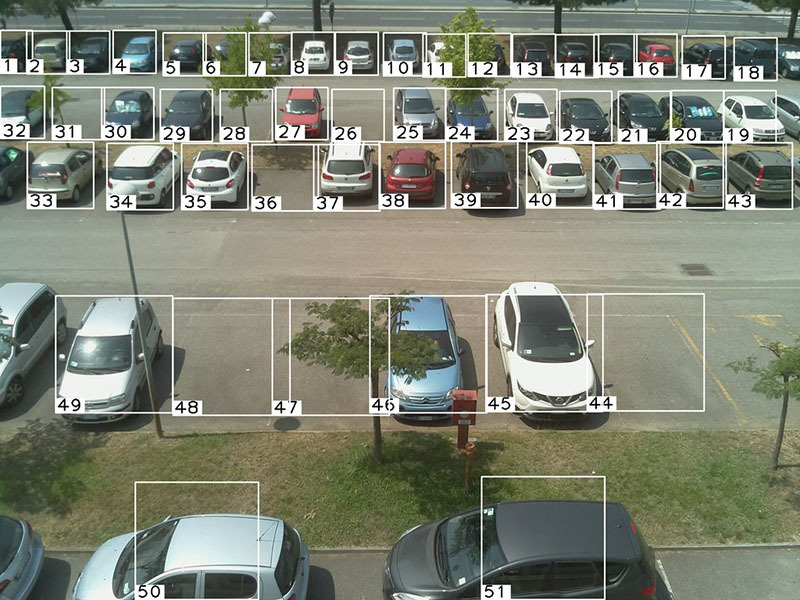
\includegraphics[width=\columnwidth]{camera-a-overview}
        \caption{Overview of CNRPark CAM A.}
        \label{fig:mini:cam-a}
    \end{subfigure} %
    \begin{subfigure}[b]{0.49\columnwidth}
        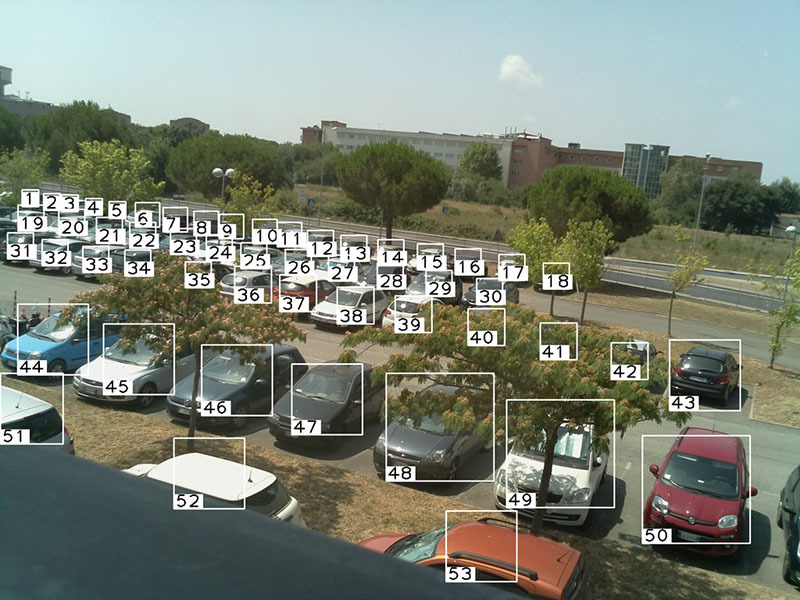
\includegraphics[width=\columnwidth]{camera-b-overview}
        \caption{Overview of CNRPark CAM B.}
        \label{fig:mini:cam-b}
    \end{subfigure}

    \begin{subfigure}[b]{0.49\columnwidth}
        \includegraphics[width=\columnwidth]{overview-cam1}
        \caption{Overview of CNRPark-EXT CAM 1.}
        \label{fig:mini:cam-1}
    \end{subfigure} %
    \begin{subfigure}[b]{0.49\columnwidth}
        \includegraphics[width=\columnwidth]{overview-cam8}
        \caption{Overview of CNRPark-EXT CAM 8.}
        \label{fig:mini:cam-8}
    \end{subfigure}
    \caption{Segmentation masks for parking slot images in the preliminary \emph{CNRPark} dataset (a-b) and in the extended \emph{CNRPark-EXT} dataset only for camera 1 (c) and 8 (d).
    \figfrom{amato2017deep}.}
    \label{fig:mini:cam-overview}
\end{figure}

\begin{figure}
\begin{subfigure}{0.25\columnwidth}%
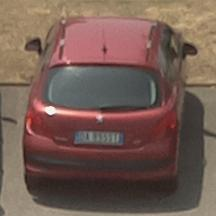
\includegraphics[width=\columnwidth]{38busy}%
\end{subfigure}%
\begin{subfigure}{0.25\columnwidth}%
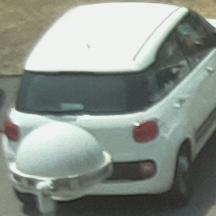
\includegraphics[width=\columnwidth]{34busy}%
\end{subfigure}%
\begin{subfigure}{0.25\columnwidth}%
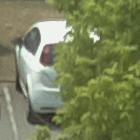
\includegraphics[width=\columnwidth]{11busy}%
\end{subfigure}%
\begin{subfigure}{0.25\columnwidth}%
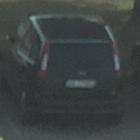
\includegraphics[width=\columnwidth]{13busy}%
\end{subfigure}

\begin{subfigure}{0.25\columnwidth}
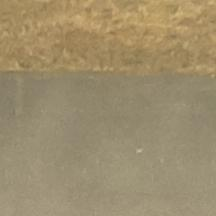
\includegraphics[width=\columnwidth]{38empty}%
\end{subfigure}%
\begin{subfigure}{0.25\columnwidth}%
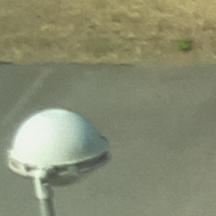
\includegraphics[width=\columnwidth]{34empty}%
\end{subfigure}%
\begin{subfigure}{0.25\columnwidth}%
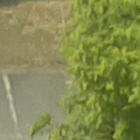
\includegraphics[width=\columnwidth]{11empty}%
\end{subfigure}%
\begin{subfigure}{0.25\columnwidth}%
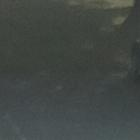
\includegraphics[width=\columnwidth]{13empty}%
\end{subfigure}
\caption{Example of segmented parking slots images under different light conditions and occlusion patterns.
The first and second rows show four slots respectively in `occupied` and `vacant` state. \figfrom{amato2017deep}.}
\label{fig:mini:slots}
\end{figure}

\paragraph{CNRPark}
In order to measure the generalization power of the proposed approach to unseen scenarios, we built a new dataset --- named \emph{CNRPark} --- collecting images from the parking lot in the campus of the National Research Council (CNR) in Pisa.
The preliminary version of this dataset --- which we refer to as CNRPark --- contains roughly $12,000$ images of slots of a part of the parking lot which were collected from 2 Raspberry Pi cameras (denoted as camera $A$ and $B$) with different perspectives and angles of view in different days of July 2015 (see \ref{fig:mini:cam-a,fig:mini:cam-b}).
Images of individual parking slots are extracted using manually-placed squared masks from the full camera frame.
Slot masks are placed to minimize the part of adjacent slots contained in the image, often limiting the area usable for classification to just a part of the entire slot.
Moreover, in many slots, occlusions by adjacent cars and obstacles (e.g., trees, lampposts) are inevitable due to the skewed field of view of the cameras;
this also involves that slots images have different sizes depending on the distance of the slot from the capturing camera.
Thus, our dataset poses additional challenges to occupancy detection methods that can be commonly found in real scenarios.
We split the dataset into two non-overlapping sets named \emph{CNRParkOdd} and \emph{CNRParkEven} respectively containing slot images having odd or even slot id.
This permitted us to test the generalization of our approach by training on some slots and test on unseen slots.

\paragraph{CNRPark-EXT}
We subsequently extended the CNRPark dataset gathering more images of the whole parking lot --- comprised of 164 parking slots --- captured by nine additional cameras from November 2015 to February 2016.
\ref{fig:mini:cam-1,fig:mini:cam-8} report the cameras with respectively the most and least skewed views.
Images were collected in multiple days spanning multiple seasons of the year, and the number of slots monitored by each camera roughly spans from 10 to 50.
To extract the images of individual slots, we followed the same strategy of CNRPark.
The extended version of the dataset --- dubbed \emph{CNRPark-EXT} -- is composed of 4,287 camera frames acquired in 23 different days, from which we obtained 144,965 manually labeled images of individual parking slots.
The added value of our dataset stands in the fact that it captures a variety of occlusion and shadow patterns, and light and weather conditions (see \ref{fig:mini:slots}) that cover more real-case scenarios with respect to existing datasets.
Slot images are grouped by camera ID, by the time of capture, and by three weather conditions --- i.e., \emph{Sunny}, \emph{Overcast}, and \emph{Rainy}.
We also provide splits for training, validation, and test sets;
we ensured that images captured in a particular day do not span more than one set.

\ref{tab:mini:datasets} reports detailed information about the composition of \emph{CNRPark}, \emph{CNRPark-EXT}, and \emph{PKLot}~\cite{de2015pklot}.
The main difference between our datasets and the existing ones can be summarized as follows.
Slot images in \emph{CNRPark-EXT} often do not cover precisely or entirely the parking slot volume, whereas in \emph{PKLot} slots are registered and straightened, resulting in a more precise coverage of the parking slot.
Moreover, \emph{CNRPark-EXT} captures heavy occlusion patterns (some slots are almost entirely covered by trees and lampposts) and lower point of views, resulting in significant occlusions due to adjacent vehicles.
Even if our dataset counts fewer images than \emph{PKLot} and has been collected from a single parking lot, we assessed through experiments that the real challenge comes from the variety of viewpoints and occlusions patterns of which our dataset is rich:
in fact, we let the \gls{cnn} to cope with these factors, resulting in a more robust classifier in real case scenarios and a reduced manual setup effort.

\begin{table}
\newcolumntype{R}{>{\raggedleft\arraybackslash}X}
% \def\arraystretch{1}
\begin{tabularx}{\linewidth}{lRRR}
\toprule
\textsc{Dataset}    & \textsc{vacant} & \textsc{occupied} & \textsc{total} \\
\midrule
%                       &               &               &                \\
%    CNRPark $A$       & 2549          & 3622          & 6171           \\
%    CNRPark $B$       & 1632          & 4781          & 6413           \\ \hline
%    CNRPark           & 4181          & 8403          & 12584          \\

     CNRPark           & 4,181          & 8,403          & 12,584          \\
     CNRPark-EXT       & 65,658         & 79,307         & 144,965         \\
     PKLot             & 337,780        & 358,119        & 695,899         \\ %\hline
%                       &               &               &                \\
%    CNRPark TRAIN     & 2201          & 3970          & 10000          \\
%    CNRPark VAL       & 1980          & 4433          & 2584           \\ \hline
%    CNRPark           & 4181          & 8403          & 12584          \\
\bottomrule
                       &               &               &                \\
\toprule
\textsc{Subset} & \textsc{vacant} & \textsc{occupied} & \textsc{total} \\ \midrule
    CNRParkOdd        & 2,201          & 3,970          & 6,171           \\
    CNRParkEven       & 1,980          & 4,433          & 6,413           \\ %hline
\midrule
     CNRPark-EXT TRAIN     & 46,877         & 47,616         & 94,493          \\
     CNRPark-EXT VAL       & 5,232          & 13,415         & 18,647          \\
     CNRPark-EXT TEST      & 13,549         & 18,276         & 31,825          \\ %\hline
%     CNRPark-EXT           & 65658         & 79307         & 144965         \\
\midrule
     CNRPark-EXT SUNNY     & 25,665         & 37,513         & 63,178          \\
     CNRPark-EXT OVCST     & 21,067         & 23,176         & 44,243          \\
     CNRPark-EXT RAINY     & 18,926         & 18,618         & 37,544          \\ %\hline
%     CNRPark-EXT           & 65658         & 79307         & 144965         \\
\midrule
     CNRPark-EXT \emph{C1}      & 6,407          & 9,308          & 15,715          \\
     CNRPark-EXT \emph{C2}       & 1,454          & 2,641          & 4,095           \\
     CNRPark-EXT \emph{C3}       & 4,101          & 5,370          & 9,471           \\
     CNRPark-EXT \emph{C4}       & 7,219          & 9,357          & 16,576          \\
     CNRPark-EXT \emph{C5}       & 9,582          & 11,256         & 20,838          \\
     CNRPark-EXT \emph{C6}       & 9,462          & 10,646         & 20,108          \\
     CNRPark-EXT \emph{C7}       & 10,595         & 10,519         & 21,114          \\
     CNRPark-EXT \emph{C8}       & 11,237         & 12,847         & 24,084          \\
     CNRPark-EXT \emph{C9}       & 5,601          & 7,363          & 12,964          \\ %\hline
%     CNRPark-EXT           & 65658         & 79307         & 144965         \\
\midrule
%					   &               &               &                \\
     PKLot2Days        & 27,314         & 41,744         & 69,058          \\
     PKLotNot2Days     & 310,466        & 316,375        & 626,841         \\ %\hline
%     PKLot             & 337780        & 358119        & 695899         \\
%                       &               &               &                \\
\midrule
     PKLot UFPR04 TRAIN& 25,894         & 23,266         & 49,160          \\
     PKLot UFPR04 TEST & 33,824         & 22,859         & 56,683          \\
     PKLot UFPR05 TRAIN& 45,759         & 48,196         & 93,955          \\
     PKLot UFPR05 TEST & 22,600         & 49,230         & 71,830          \\
     PKLot PUC TRAIN   & 114,424        & 106,334        & 220,758         \\
     PKLot PUC TEST    & 115,616        & 87,895         & 203,511         \\ %\hline
%     PKLot             & 337780        & 358119        & 695899         \\
%                       &               &               &                \\
\midrule
     PKLot TRAIN       & 27,314         & 41,744         & 105,843         \\
     PKLot VAL         & 54,909         & 47,453         & 165,785         \\
     PKLot TEST        & 275,894        & 248,583        & 424,269         \\ %\hline
%     PKLot             & 337780        & 358119        & 695899         \\
\bottomrule
\end{tabularx}
\caption{Details of datasets and their subsets used in the experiments.
Values refer to the number of slot images contained in every dataset or subset.}
\label{tab:mini:datasets}
\end{table}

\section{Evaluation}
\label{sec:mini:evaluation}

In this section, we present the experimental evaluation and discuss the obtained results.
Our investigation focused on getting insight on three main aspects of the proposed solution that can be summarized by the following questions:
\begin{enumerate}
\item How does our reduced classifier compare against state-of-the-art approaches?
\item How much the generalization performance degrades when using our reduced model instead of the original AlexNet architecture?
\item How much the proposed solution for visual occupancy detection is robust to weather and viewpoint changes?
\end{enumerate}

To answer these questions, we extensively evaluated our approach using the two datasets described in \ref{sec:mini:datasets}, i.e., PKLot and CNRPark-EXT.
We performed experiments by splitting the datasets into several subsets that we will describe in the following subsections.
Details about data splits are summarized in \ref{tab:mini:datasets}.
The adoption of multiple methods on multiple datasets also permitted us to compare the quality of our newly collected dataset for learning to detect occupancy detection robustly in real scenarios.

\subsection{Comparison with the State of the Art}
\label{sub:mini:sota}

We compared mAlexNet against the state-of-the-art visual occupancy detection system proposed by \citet{de2015pklot}, which relies on \glspl{svm} classifiers with RBF kernels defined over handcrafted textural features.
Specifically, histograms of \gls{lbp}, \gls{lpq} features and their variations~\cite{ojala2002multiresolution, ojansivu2008blur, rahtu2012local} have been tested as input features of the \gls{svm}.
\Glspl{svm} are calibrated to output the probability of a slot to be occupied.
The authors also showed an improved classification performance  using ensembles of \gls{svm} classifiers each defined on a particular textural feature:
probability values are fused using simple aggregation functions, such as \emph{Max} and \emph{Mean}, to obtain the final decision for an image slot.

We followed the experimental protocol described in~\cite{de2015pklot}.
We split images from each camera of the PKLot dataset (UFPR04, UFPR05, and PUC) into a training and test set with roughly a 50\%--50\% proportion;
for a fair evaluation, we ensured that images collected in a particular day do not appear in both training and test set.
We then trained both mAlexNet and the \glspl{svm} on each of the three training set, and tested on all the available test sets.
%
%Similarly, we also repeated the same protocol with our preliminary CNRPark dataset.
%We split CNRPark into two subsets --- CNRParkEven and CNRParkOdd --- respectively containing images of slots having even and odd IDs.
%We train both \glspl{svm} and mAlexNet on one subset and test on the other, and vice-versa.

For each experiment, we evaluated the prediction obtained for the test set by measuring the percentage error (\textbf{Err. \%}), defined as $100 \cdot (1 - \text{Accuracy})$, and the \gls{roc} \textbf{\gls{auc}}.
The former gave us an overall evaluation of the systems assuming a slot is occupied if the probability is above $0.5$, while the latter summarized the behavior of the systems independently from the probability threshold chosen.


\paragraph{Training and implementation details for mAlexNet}
Input images were squashed to a resolution of $256\times256$ before being fed to the network.
During the training phase, we performed data augmentation by taking a $224\times224$ random crop of the resized image and flipping it horizontally with probability $\sfrac{1}{2}$.
In the test phase, images were resized to $224\times224$ resolution, and no flipping was performed.
We trained all the mAlexNet models with \gls{sgd} with momentum for 18 epochs, with a learning rate of 0.01 halved every 6 epochs, a batch size of 64, a momentum of 0.9, and a weight decay of $5\times 10^{-4}$;
due to the low model complexity, no dropout regularization was used.
To avoid overfitting on the test set, we validated our models at each training epoch by evaluating it on a validation set.
As validation sets, we used the training splits of the PKLot cameras --- e.g., when testing on the PUC test subset, we use the PUC training subset as validation set.
We chose as the final model for a particular dataset the one which performs best on the validation test.

\paragraph{Training and implementation details for \glspl{svm}}
To train the \glspl{svm}, we employed the procedure and the hyper-parameters as described by \citet{de2015pklot} here summarized.
We extracted \gls{lbp}-type features with a radius of 1 and 8 neighbors.
\gls{lpq} features are extracted using a window size of 3x3.
The $C$ and $\gamma$ parameters of \glspl{svm} are chosen with grid search and 5-fold cross-validation on the training set.
We chose the parameters $(C,\gamma)$ obtaining the best 5-fold accuracy, i.e., the best accuracy obtained classifying each fold of the dataset with the model trained on the other folds.
The final SVM was then trained on the entire training set using the chosen parameters and evaluated on the test set.
We followed the same strategy used in~\cite{de2015pklot} to obtain a probabilistic score from the output of the \gls{svm}, which evaluates the posterior probability fitting a sigmoid function with two parameters~\cite{platt1999probabilistic}.

\begin{table}
    \newcolumntype{C}{>{\centering\arraybackslash}X}
    \begin{tabularx}{\linewidth}{lcX}
        \toprule
        \textsc{Method} & \textsc{Input Dim.}     & \textsc{Input Description} \\
        \midrule
        mAlexNet         & $224\times 224\times 3$ & a 224x224 RGB image \\
        SVM + LBP        & $256$                     & histograms of classical \acrfull{lbp}~\cite{ojala2002multiresolution} \\
        SVM + LBPu       & $59$                      & histograms of uniform LBP~\cite{ojala2002multiresolution} \\
        SVM + LBPri      & $36$                      & histograms of rotational invariant LBP~\cite{ojala2002multiresolution}  \\
        SVM + LBPuri     & $10$                      & histograms of uniform and rotational invariant LBP~\cite{ojala2002multiresolution} \\
        SVM + LPQu       & $256$                     & histograms of \acrfull{lpq} (uniform initialization)~\cite{ojansivu2008blur} \\
        SVM + LPQg       & $256$                     & histograms of LPQ (gaussian initialization)~\cite{rahtu2012local} \\
        SVM + LPQgd      & $256$                     & histograms of LPQ (gaussian derivative initialization)~\cite{rahtu2012local} \\
        \bottomrule
     \end{tabularx}
     \caption{Summary of state-of-the-art methods compared against our approach for parking slot occupancy detection.}
     \label{tab:mini:methods}
\end{table}

\begin{table}
	\newcolumntype{R}{>{\raggedleft\arraybackslash}X}

	\begin{tabularx}{\linewidth}{lRRRRRR}
	\toprule
	\textsc{Method}               & \multicolumn{2}{c}{\textsc{UFPR04}} & \multicolumn{2}{c}{\textsc{UFPR05}}  & \multicolumn{2}{c}{\textsc{PUC}}  \\
								    \cmidrule(lr){2-3}  \cmidrule(lr){4-5}   \cmidrule(lr){6-7}
	\textbf{Train on UFPR04}      & \textbf{Err. \%} & \textbf{AUC} & \textbf{Err. \%} & \textbf{AUC} & \textbf{Err. \%} & \textbf{AUC} \\
	\midrule
	mAlexNet                      & 0.46 & 0.99      & 6.71  & 0.99    & 1.73  & 0.99 \\
	LPQu / LPQg / LPQg*           & 0.45 & 0.99      & 15.08 & 0.94    & 15.75 & 0.94 \\
	Mean / Max / Max Ensemble*    & 0.36 & 0.99      & 11.67 & 0.95    & 11.60 & 0.95 \\
	\midrule
	\textbf{Train on UFPR05}      & \textbf{Err. \%} & \textbf{AUC} & \textbf{Err. \%} & \textbf{AUC} & \textbf{Err. \%} & \textbf{AUC} \\
	\midrule
	mAlexNet                      &  6.31 & 0.98     & 0.51 & 0.99     & 7.28  & 0.98 \\
	LPQgd / LPQu / LPQu*          & 14.24 & 0.93     & 1.10 & 0.99     & 12.26 & 0.94 \\
	Mean  Ensemble*               & 14.47 & 0.95     & 0.70 & 0.99     & 10.17 & 0.97 \\
	\midrule
	\textbf{Train on PUC}         & \textbf{Err. \%} & \textbf{AUC} & \textbf{Err. \%} & \textbf{AUC} & \textbf{Err. \%} & \textbf{AUC} \\
	\midrule
	mAlexNet                      &  1.97 & 0.99     & 4.00  & 0.99    & 0.10 & 0.99 \\
	LPQg / LBPri / LPQu*          & 12.85 & 0.94     & 17.22 & 0.91    & 0.42 & 0.99 \\
	Mean  Ensemble*               & 11.12 & 0.95     & 15.80 & 0.91    & 0.39 & 0.99 \\
	\bottomrule
	\end{tabularx}

%	\begin{tabularx}{\linewidth}{XRRRR}
%	\toprule
%	                              & \multicolumn{2}{c}{\textsc{CNRParkEven}} & \multicolumn{2}{c}{\textsc{CNRParkOdd}} \\
%	\textsc{Method}               & \multicolumn{2}{c}{\textbf{\small Train on CNRParkOdd}} & \multicolumn{2}{c}{\textbf{\small Train on CNRParkEven}} \\
%									\cmidrule(lr){2-3}                         \cmidrule(lr){4-5}
%								  & \textbf{Err. \%} & \textbf{AUC} & \textbf{Err. \%} & \textbf{AUC} \\
%	\midrule
%	mAlexNet                      & 9.87 & 0.94 & 9.29 & 0.92  \\
%	LPQgd / LBP*                  & 12.35 & 0.95 & 12.79 & 0.92 \\
%	\bottomrule
%	\end{tabularx}

	\caption{Comparison of mAlexNet against state-of-the-art approaches presented by \citet{de2015pklot}.}
	\label{tab:mini:net-vs-svms}
\end{table}

A summary of the compared methods is reported in \ref{tab:mini:methods}, and results are reported in \ref{tab:mini:net-vs-svms}.
For simplicity, we report for each experiment only the variant of \gls{lbp} or \gls{lpq} that yielded the best performance on each subset, and for ensembles, we report the best performing aggregation function.
We can notice that mAlexNet generally perform better than other compared methods in terms of both percentage error and AUC.
All the methods perform well when training and test images come from the same camera;
in fact, most of them reach a classification error less than 1\%.
However, our \gls{cnn}-based solution exhibits a stronger generalization power, reaching errors 3--10\% lower when training and test images come from different cameras.
% In fact, mAlexNet reaches accuracy values of 98.27\% in the UFPR04/PUC training/test set configuration.
% This is roughly 10\% more accurate than the best compared method, that is \emph{Max Ensemble}, which reaches 88.40 \%.

To stress test the generalization capabilities, we also performed experiments when training and test sets come from a completely different dataset, which is a common assumption in the setup and deployment of real systems.
We used both PKLot and CNRPark dataset respectively as training and test set, and vice-versa.
To reduce training times of \glspl{svm}, we used a smaller subset of PKLot as training set --- named PKLot2Days --- obtained by selecting images captured in the first two days in chronological order for each camera (UFPR04, UFPR05, and PUC) and each weather condition (SUNNY, OVERCAST, RAINY) available.
The test phase was still performed on the whole PKLot dataset.

\begin{table}
  \newcolumntype{R}{>{\raggedleft\arraybackslash}X}
  \begin{tabularx}{\linewidth}{lRRRR}
  \toprule
                                & \multicolumn{2}{c}{\textsc{CNRPark}} & \multicolumn{2}{c}{\textsc{PKLot}} \\
  \textsc{Method}               & \multicolumn{2}{c}{\textbf{\small Train on PKLot2Days}} & \multicolumn{2}{c}{\textbf{\small Train on CNRPark}} \\
                                  \cmidrule(lr){2-3}                              \cmidrule(lr){4-5}
                                & \textbf{Err. \%} & \textbf{AUC}               & \textbf{Err. \%} & \textbf{AUC} \\
  \midrule
  mAlexNet                      & 17.12            & 0.899                      &  9.62            & 0.989 \\
  LPQu                          & 35.36            & 0.447                      & 60.18            & 0.743 \\
  LPQgd                         & 38.26            & 0.465                      & 59.01            & 0.601 \\
  LPQg                          & 36.16            & 0.450                      & 56.19            & 0.599 \\
  LBPuri                        & 34.69            & 0.580                      & 50.26            & 0.496 \\
  LBPu                          & 35.73            & 0.506                      & 53.33            & 0.450 \\
  LBPri                         & 35.80            & 0.556                      & 51.28            & 0.405 \\
  LBP                           & 36.87            & 0.491                      & 47.12            & 0.391 \\
  \bottomrule
  \end{tabularx}

  \caption{Cross-dataset experiments performed to stress test the generalization performance of compared methods.}
  \label{tab:mini:x-dataset}
\end{table}

Results in \ref{tab:mini:x-dataset} clearly show how features learned by the \gls{cnn} are more transferable to different domains with respect to the manually engineered textural features.
Moreover, as expected, classifying the CNRPark dataset while training on PKLot is more challenging than its counterpart.
Despite being smaller, the greater variability and the additional occlusion patterns captured by our dataset comprises a richer training set for learning-based methods.
In fact, the whole PKLot can be annotated with roughly 10\% error while training on CNRPark which contains 60$\times$ fewer images.
Again, mAlexNet still outperforms the other compared classifiers in this configuration.
As stated by \citet{de2015pklot}, we did not observed an absolute best textural feature among the tested one.
% However, we noticed that in most of the cases, LPQu and LPQg (Local Phase Quantization with respectively uniform and Gaussian initialization), give better performance.
% We noticed in their results that taking the mean of the confidence coming from different classifiers (to which we refer with \emph{Mean Ensemble}) usually improves the performance.

% We also report the experiments performed in a preliminary work~\cite{amato2016car} in which we
% compared mAlexNet to the techniques proposed in~\cite{de2015pklot} using \emph{CNRPark} dataset.
% For each experiment, we report only the variant of LBP or LPQ that yielded the best performance.

\subsection{Evaluation of the Generalization: Parking Lot}
\label{subsec:mini:generalization}

In this section, we describe the experiments and results we performed to compare the generalization performance of our reduced \gls{cnn} architecture against the original AlexNet architecture.

To measure the generalization performance, we trained both models on a dataset, and we evaluated the trained models on a different one, in which images are coming from a different parking lot and have different camera height and pose.
We performed multiple experiments using different sets of images also to measure the generalization power obtained by datasets with different degree of variability.
As training sets, we separately employed \emph{CNRPark}, \emph{CNRPark} plus cameras \emph{C1} and \emph{C8} of \emph{CNRPark-EXT}, \emph{CNRPark-EXT}, and \emph{PKLot}.
Validation was performed on the corresponding validation sets, while evaluation metrics --- i.e., percentage error and \gls{auc} --- are reported for CNRPark-EXT and PKLot test sets.
The set composed by \emph{CNRPark} plus cameras \emph{C1} and \emph{C8} of \emph{CNRPark-EXT} was chosen to built a balanced set of different viewpoints.
While \emph{CNRPark-EXT} is comprised of nine different cameras, most of them share the same frontal viewpoint of the parking lot.
Thus, we selected \emph{C1} and \emph{C8} --- which have the most divergent views of the parking lot --- and we combined them with CNRPark, which is composed by other two different viewpoints (see \ref{fig:mini:cam-overview}).

We trained all the models for 6 epochs, with a learning rate of $8e^{-4}$, which is multiplied by 0.75 every 2 epochs.
Other hyper-parameters are the following: batch size 64, momentum 0.9, and weight decay $5e^{-4}$.
As the final models, we chose the ones obtaining the best performance on the validation sets.
Details about the subsets used in these experiments are reported in \ref{tab:mini:datasets}.

% In experiments 1.1 and 1.2, we measured how much predictive power both models can obtain from the \emph{PKLot} dataset.
% We splitted both the \emph{PKLot} and \emph{CNRPark-EXT} datasets in TRAIN/VAL/TEST subsets picking images from different days from all the weather conditions.
% We trained both networks on the \emph{PKLot TRAIN}, using use \emph{PKLot VAL} and \emph{CNRPark-EXT VAL} as validation sets.
% We then computed the accuracy of those two trained models on \emph{PKLot TEST} and \emph{CNRPark-EXT TEST}.

% We then measured the informativeness of our preliminary dataset \emph{CNRPark}, following the same methodology for experiments 2.1 and 2.2.
% We trained both models using \emph{CNRPark} as training set, \emph{CNRPark-EXT VAL} and \emph{PKLot VAL} as validation sets, and we tested on \emph{CNRPark-EXT TEST} and \emph{PKLot TEST}.

% In experiments 3.1 and 3.2, we replicated experiments 2.1 and 2.2, using the extended dataset \emph{CNRPark-EXT}.
% The training set is composed by the whole \emph{CNRPark} plus \emph{CNRPark-EXT TRAIN}, named \emph{CNRPark+EXT TRAIN} for brevity.
% % \emph{CNRPark-EXT VAL} was used as validation set instead of \emph{CNRPark VAL}.

% In experiments 4.1 and 4.2, we replicated experiments 3.1 and 3.2, using a more balanced training set in terms of viewpoints.
% In \emph{CNRPark+EXT TRAIN}, the majority of the images are captured  from a frontal viewpoint.
% We selected only two cameras from \emph{CNRPark-EXT TRAIN}, camera 1 and camera 8, that have the most different viewpoints of the parking lot.
% Thus we obtained a balanced number of images from different viewpoints.
% We added those images to \emph{CNRPark}, forming a new balanced training set, named \emph{CNRPark+EXT TRAIN C1-C8}.

\begin{table}
  \newcolumntype{R}{>{\raggedleft\arraybackslash}X}

  \begin{tabularx}{\linewidth}{lRRRR}
  \toprule
  \textsc{Method}               & \multicolumn{2}{c}{\textsc{CNRPark-EXT TEST}} & \multicolumn{2}{c}{\textsc{PKLot TEST}} \\
                                  \cmidrule(lr){2-3}                              \cmidrule(lr){4-5}
  \textbf{Train on CNRPark}     & \textbf{Err. \%} & \textbf{AUC}               & \textbf{Err. \%} & \textbf{AUC} \\
  \midrule
  mAlexNet                      & 6.48             & 0.9838                     & 4.72             & 0.9916 \\
  AlexNet                       & 6.37             & 0.9877                     & 4.40             & 0.9910 \\
  \midrule

  \textbf{Train on CNRPark+EXT TRAIN C1,C8} & \textbf{Err. \%} & \textbf{AUC}   & \textbf{Err. \%} & \textbf{AUC} \\
  \midrule
  mAlexNet                      & 4.12             & 0.9937                     & 9.52             & 0.9738 \\
  AlexNet                       & 3.15             & 0.9957                     & 3.49             & 0.9937 \\
  \midrule

  \textbf{Train on CNRPark+EXT TRAIN} & \textbf{Err. \%} & \textbf{AUC}         & \textbf{Err. \%} & \textbf{AUC} \\
  \midrule
  mAlexNet                      & 2.29             & 0.9967                     & 15.47            & 0.9699 \\
  AlexNet                       & 2.00             & 0.9974                     &  6.30            & 0.9923 \\
  \midrule

  \textbf{Train on PKLot TRAIN} & \textbf{Err. \%} & \textbf{AUC}    & \textbf{Err. \%} & \textbf{AUC} \\
  \midrule
  mAlexNet                      & 16.17            & 0.9139                     & 1.93             & 0.9967 \\
  AlexNet                       &  9.48            & 0.9684                     & 1.19             & 0.9984 \\
  \bottomrule
  \end{tabularx}

  \caption{Experiments performed to test the generalization performance of mAlexNet and AlexNet.
  Accuracies on test sets are reported, for each combination of model, training set, and test set.}
  \label{tab:mini:malex-vs-alex}
\end{table}

Results are reported in \ref{tab:mini:malex-vs-alex}.
We can notice that our reduced architecture does not suffer from a performance degradation with respect to the original AlexNet when data comes from the same domain;
in fact, the percentage errors of both models differ at most of 1\% in all experiments where training and test subsets are taken from the same dataset.
When training and test are performed on different datasets, AlexNet reaches higher accuracy values.
It is clear that the reduced architecture limits the degree of generalization the model can reach;
when using a viewpoint-balanced training set (i.e., \emph{CNRPark} and \emph{Train on CNRPark+EXT TRAIN C1,C8}), AlexNet reaches a percentage error on \emph{PKLot} of 3.49\%, while our method performs worse still obtaining less than 10\% error.

In the best case, there is practically no difference between the two methods, while in the worst case, we measured a difference of $\sim 9\%$ with respect to mAlexNet.
A bigger model offers a greater generalization performance at the cost of more resources needed:
the computation time for mAlexNet --- measured on the Raspberry Pi model B --- allows performing a classification in roughly 300ms, while AlexNet takes roughly 20s.

\subsection{Evaluation of the Generalization: Viewpoint and Weather}

%Errors in the occupancy detection of parking spaces are due to many reasons.
%For instance, the lighting condition changes during different periods of the year;
%moreover, occlusions and reflection patterns might introduce a fixed source of error.
%The weather condition might produce significant illumination changes as well.
%During a rainy weather, puddles and wet floor create textural patterns that may lead to a misclassification.
%Sunbeams can create reflections on the car's windscreen or on water, covering the majority of the images with saturated patterns.
%As we discussed in previous experiments, errors might also be due to low generalization properties of the classifier.
%When a classifier does not generalize well, it works well just in the conditions where it was trained.
%For instance, a bad classifier trained on a certain point of view of the parking lot, does not work well when tested with images coming from a camera seeing the parking lot from a different point of view.

The source of errors in classifiers for visual occupancy detection is manifold.
The majority of errors comes from illumination changes due to variable weather and seasonal light changes;
examples of such conditions are cloud shadows, puddles and wet ground, sun reflections, etc.
Moreover, significant viewpoint changes between training data and real data is another suitable cause of performance degradation.

We measured the robustness of our approach to these scenarios performing \emph{inter-camera} and \emph{inter-weather} experiments.
With the former, we indicate experiments where we train on a particular viewpoint and test on other unseen viewpoints, while with the latter, we indicate experiments where we train using images collected during a particular weather condition --- sunny, overcast, or rainy ---, and we test on the others.

For both experiments, we employed our extended \emph{CNRPark-EXT} dataset.
For inter-camera experiments, we trained mAlexNet using images of one camera among the nine available, and measured the accuracy obtained on images coming from the other cameras.
We repeated this experiment using both the cameras with most and less skewed viewpoints (respectively \emph{C1} and \emph{C8}) to analyze the classifier robustness to challenging viewpoint changes.
For inter-weather experiments, we performed three experiments training respectively on \emph{CNRPark-EXT SUNNY}, \emph{OVERCAST}, and \emph{RAINY} subsets and evaluating the obtained classifiers on the other weather conditions.
For both kind of experiments, we report also the performance evaluated on the PKLot dataset for completeness.
The training procedure and hyperparameters strictly follow the one described in \ref{subsec:mini:generalization}.

\begin{table}
\newcolumntype{R}{>{\raggedleft\arraybackslash}X}
\begin{tabularx}{\linewidth}{Xrrrrrrrrrr}
\toprule
\textsc{Train Set} &   \textsc{C1} &   \textsc{C2} &   \textsc{C3} &   \textsc{C4} &   \textsc{C5} &   \textsc{C6} &   \textsc{C7} &   \textsc{C8} &   \textsc{C9} & \textsc{PKLot} \\
                   \cmidrule(lr){2-2} \cmidrule(lr){3-3} \cmidrule(lr){4-4} \cmidrule(lr){5-5} \cmidrule(lr){6-6} \cmidrule(lr){7-7} \cmidrule(lr){8-8} \cmidrule(lr){9-9} \cmidrule(lr){10-10} \cmidrule(lr){11-11}
CNRPark-EXT C1 &    - & 5.15 & 6.89 & 4.00 & 4.09 & 4.39 & 8.57 & 5.39 & 9.04 & 26.92 \\
CNRPark-EXT C8 & 7.61 & 5.49 & 6.34 & 2.47 & 2.07 & 2.32 & 6.47 &    - & 5.35 &  4.51 \\
\bottomrule
\end{tabularx}
\caption{Results of inter-camera experiments in terms of accuracy obtained when training mAlexNet on camera 1 and camera 8.}
\label{tab:mini:inter-camera}
% ALTERNATIVE FIG:
% \begin{figure}
% \includegraphics[width=\linewidth]{inter-camera}
% \caption{Results of inter-camera experiments in terms of accuracy obtained when training mAlexNet on camera 1 (in blue), and on camera 8 (in red).}
% \label{fig:mini:inter-camera}
% \end{figure}
\end{table}

\begin{table}
\newcolumntype{R}{>{\raggedleft\arraybackslash}X}
\begin{tabularx}{\linewidth}{lRRRR}
\toprule
\textsc{Train Set} & \textsc{Sunny} & \textsc{Overcast} & \textsc{Rainy} & \textsc{PKLot} \\
                     \cmidrule(lr){2-2} \cmidrule(lr){3-3} \cmidrule(lr){4-4} \cmidrule(lr){5-5}
CNRPark-EXT SUNNY    &    - & 2.20  & 4.21 & 17.01 \\
CNRPark-EXT OVERCAST & 8.37 &    -  & 5.32 & 20.51 \\
CNRPark-EXT RAINY    & 6.47 & 1.73  &    - &  9.42 \\
\bottomrule
\end{tabularx}
\caption{Results of inter-weather experiments in terms of accuracy obtained when training on a sunny, overcast, or rainy weather.}
\label{tab:mini:inter-weather}
% ALTERNATIVE FIG:
% \begin{figure}[t]
% \includegraphics[width=\columnwidth]{inter-weather}
% \caption{Results of inter-weather experiments in terms of accuracy obtained when training on a sunny (in blue), overcast (in red), or rainy (in yellow) weather.}
% \label{fig:inter-weather}
% \end{figure}
\end{table}

\ref{tab:mini:inter-camera,tab:mini:inter-weather} respectively report the percentage classification error values obtained in \emph{inter-camera} and \emph{inter-weather} experiments.
% The histograms compare the accuracy of a classifier trained on a specific scenario (a specific camera or a specific whether condition) when tested on all other possible scenarios.

In \emph{inter-camera} experiments, the model trained on \emph{C8} --- which has a clean and central view of the parking lot --- exhibited the best performance on most of the other cameras since their viewpoint do not differ significantly;
the worst performance among all cameras is obtained on \emph{C1} --- which mainly captures partially occluded images and has the most skewed viewpoint that differs the most from \emph{C8}.
For the same reason, the model trained on \emph{C1} has worse performance but still can reach less than 10\% error on cameras coming from the same dataset.
The PKLot dataset is mainly composed of images with no occlusions and with a central and vertical view of the parking lots, and thus it is better classified by the model trained on \emph{C8}.

In \emph{inter-weather} experiments, we observed a strong generalization pattern.
Moreover, the performance degradation is directly related to the difference between training and testing weather conditions.
For example, when training on ``sunny'' images, we achieve better performance on ``overcast'' images than ``rainy'' ones.
Similarly, when training on ``rainy'' images, the model is more accurate on ``overcast' images than ``sunny'' ones.
Results on the \emph{PKLot} dataset showed that light conditions play an important role in the classification performance;
we noticed that these are similar between images in the \emph{PKLot} dataset and ``rainy'' images, which justifies the lower percentage error in the results.

\section{Deployment on CNR Pisa Parking Lot}
\label{sec:mini:deployment}

\begin{figure}
	\centering
    \begin{subfigure}{0.48\columnwidth}
		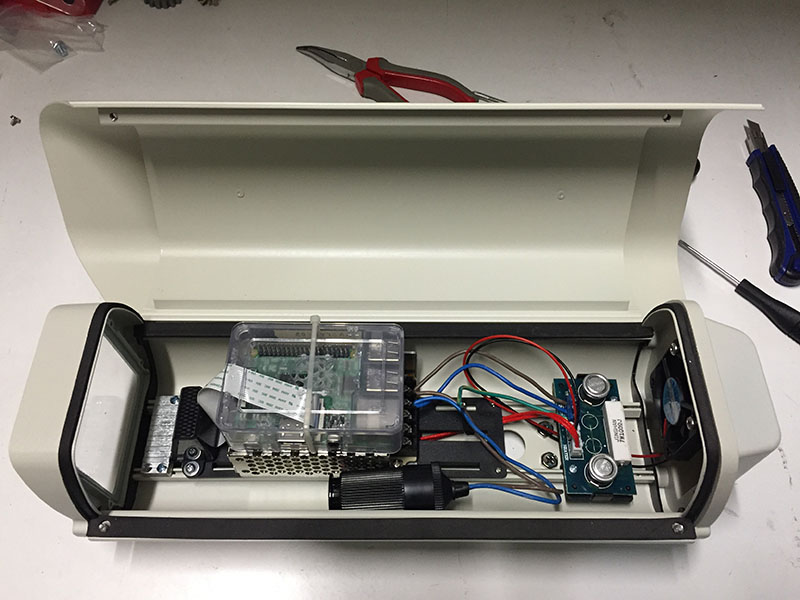
\includegraphics[width=\columnwidth]{camera_inside}
        \caption{A Raspberry Pi smart camera inside its camera box.}
	\end{subfigure} %
    \begin{subfigure}{0.48\columnwidth}
		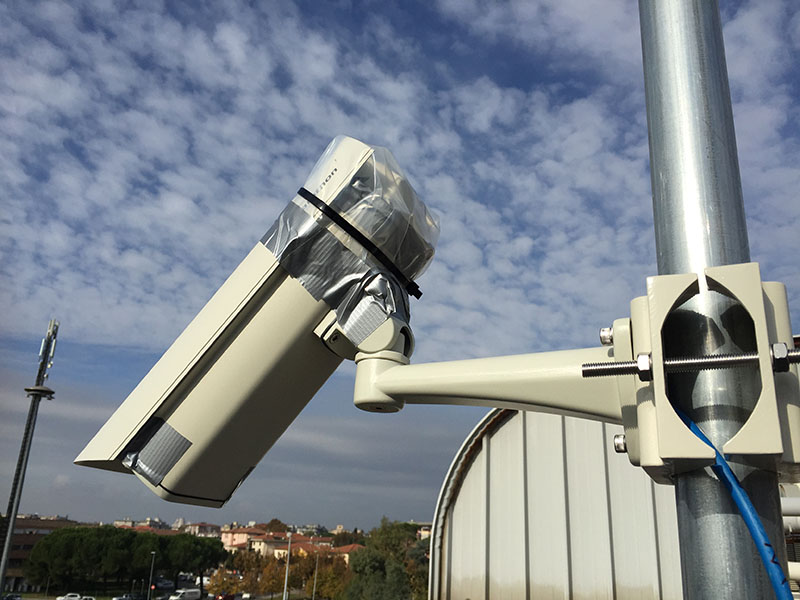
\includegraphics[width=\columnwidth]{camera_box}
        \caption{The complete camera box used mounted on the roof of the building.}
	\end{subfigure}
	\caption{Example of camera box mounted in the deployment of the CNR Pisa parking lot. \figfrom{amato2017deep}.}
	\label{fig:mini:camera-box}
\end{figure}

\begin{figure}
	\centering
	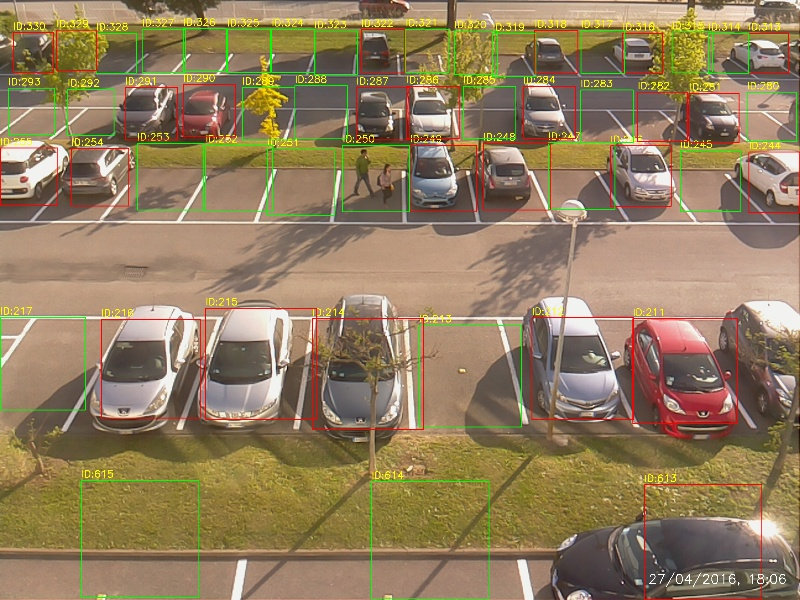
\includegraphics[width=\columnwidth,trim={0 0 0 3.5ex},clip]{detection-example}
    \caption{Example of classification of a portion of the parking lot. \figfrom{amato2017deep}.}
	\label{fig:mini:detection-example}
\end{figure}

In this section, we describe the details of the deployment of a prototype of our proposed solution for parking lot visual occupancy detection in the campus of the National Research Council (CNR) in Pisa.

We deployed nine smart cameras on the roof of the building in front of a section of the campus parking lot.
Each smart camera is built from a Raspberry Pi 2 model B equipped with a standard Raspberry Pi camera module and mounted on an outdoor camera box (see \ref{fig:mini:camera-box}).
The total cost for a single camera is roughly 80\euro.
Hardware and software details are briefly reported for completeness.
The smart cameras are equipped with an ARM Cortex-A7 CPU, 1GB RAM DDR2, and a 32GB micro SD card for storage.
The camera module is a 5MP fixed-focus camera that supports 1080p30, 720p60 and VGA90 video modes, as well as still captures.
The view angles of the camera are 53.50$^{\circ}$ horizontally and 41.41$^{\circ}$ vertically.
We capture still pictures at a full-sensor resolution of $2592 \times 1944$ pixels.
We used the OpenCV\footnote{http://opencv.org/} library to elaborate the frames acquired by the cameras, and Caffe~\cite{jia2014caffe} to train and use neural networks.

Periodically, cameras capture an image of a portion of the parking lot, segment individual slots using manually defined masks, and determine the occupancy status for each slot using the \gls{cnn} trained offline.
\ref{fig:mini:detection-example} shows an example of the occupancy detection performed by one camera in which common challenging aspects --- such as shadows, obstacles (trees or lamps) or even people occupying the parking slots --- are correctly managed.
In total, the cameras monitor 164 parking spaces organized in five rows, the first comprised of 18 parking spaces each, and the others by 35 parking slots each.
The number of parking slots monitored by each camera spans from 20 to more than 50, roughly, depending on the position of the parking slots with respect to the building on which cameras are mounted.
In fact, some cameras are dedicated to monitoring most of the parking spaces closest to the building, while further spaces are monitored by multiple cameras.
We exploit the redundancy offered by multiple cameras to reduce the classification uncertainty when possible.
We combine the predictions of slots monitored by more than one camera by manually assigning weights to each (slot, camera) couple that represent the quality of the camera view for that particular slot.
As the correct prediction for a slot, we take the one with highest weighted confidence.

The predicted occupancy status for each slot is submitted to a server for visualization and counting purposes.

% A key aspect of the proposed system is its decentralized approach
% and the delegation of the parking decision to the smart cameras
% themselves. This solution has the clear advantage of being scalable
% as it requires no additional elaboration on the server side. In a
% centralized solution images of the parking at high resolution (of
% about 3MB) should be sent to the server which would thus become a
% bottleneck and a single point of failure. Moreover, the network may
% be easily congested with increasing number of parking lots to be monitored.

\section{Summary}
\label{sec:mini:conclusions}

In this chapter, we proposed and evaluated a reduced \acrlong{cnn} architecture for image classification that enables smart vision applications in embedded devices.
In the scope of visual parking lot occupancy detection, we defined mAlexNet, a reduced version of the famous AlexNet classifier, which is obtained by pruning layers and reducing the number of parameters of the original architecture.
Experiments on public datasets showed that our proposed architecture outperforms state-of-the-art approaches for visual parking lot occupancy detection based on shallow models and handcrafted features while requiring a computational budget suitable for embedded devices.
Specifically, our architecture exhibited very high accuracies even in the presence of challenging light conditions variation, shadows, and partial occlusions.
Moreover, multi-dataset experiments showed that the architectural reduction does not introduce a performance degradation in real scenarios, and it produces only a slight acceptable degradation of the generalization capability, i.e., the ability to classify images coming from different parking lots with different imaging conditions.

We tested our approach on a real scenario in the parking lot of the campus of the CNR Area in Pisa.
We deployed a decentralized system comprised of nine smart cameras which monitors multiple slots and perform the occupancy detection for each slot on board.
The delegation of parking slot occupancy detection to smart cameras provides a twofold advantage.
First, with a cost of a single camera (roughly 80\euro), we can monitor at most 50 slots in our configuration, drastically reducing the cost per single slot that is nearly 100\euro{} for magnetic ground sensors while maintaining the same level of accuracy.
Second, the decentralized nature of our solution enables a higher degree of scalability, since there is no need for a central server to analyze images and high bandwidth to transfer them.
Besides, the flexibility of the infrastructure does not limit the applications only to occupancy detection;
the spare computational resources can be used to perform other analyses such as video surveillance activities.

As a further contribution, we collected and made publicly available \emph{CNRPark-EXT}, a dataset containing images of a real parking lot taken by nine smart cameras, in different days, with different weather and light conditions.
\emph{CNRPark-EXT} covers a high variability of occlusions, point of views, light and weather conditions, which we experimentally demonstrated being essential for the robustness and generalization of occupancy detection systems.
This makes the dataset more compatible with real scenarios of outdoor parking lots, and represents a good complement to other publicly available datasets, for more reliable assessments.

%==========================

% \emph{mLeNet} is based on LeNet-5, proposed by~\cite{lecun1998gradient}, having two convolutional layers followed by max pooling and two fully connected layers.
% The first layer (\emph{conv1}) is similar to the one proposed by~\cite{krizhevsky2012imagenet} to be more suitable for a 224x224x3 input image.
% Layers \emph{conv2} and \emph{fc4} have a reduced number of filters and neurons with respect to~\cite{lecun1998gradient} to better suit a binary classification task without overfitting.
% For \emph{fc5}, the last Gaussian RBF (radial basis function) layer is replaced with a classical inner product layer and a 2-way soft max classifier.

% Unlike~\cite{krizhevsky2012imagenet} and~\cite{lecun1998gradient}, both  architectures have a dense connection between convolutional layers.

% We used the Caffe framework~\cite{jia2014caffe} to train the neural network and to initialize the classifier.

% We first compared the two proposed CNN architectures to select the one that offers the best performance.
% Afterwards, we compared our approach against other state-of-the-art methods.
% Finally, we performed experiments to analyze the difference between our CNN architecture.

% \subsection{Assessment of the Proposed CNNs}

% \noindent In order to assess the performance of the two CNN architectures
% mAlexNet and \emph{mLeNet}, presented in Section
% \ref{sec:occupancy-detection}, we performed experiments using the
% \emph{CNRPark} dataset, considering two possible application
% scenarios:
% % a \emph{single camera scenario}, in which train and test data come from the same viewpoint, and
% % a \emph{multiple camera scenario}, in which training data and test data come from
% % different viewpoints.
% %
% \begin{inparaenum}[\itshape a\upshape)]
%   \item \emph{single camera scenario}, in which train and test data come from
%   the same viewpoint,
%   \item \emph{multiple camera scenario}, in which train data and
%   test data come from different viewpoints.
% \end{inparaenum}

% %Experiments are performed offline using the manually labeled data generated as
% %described in Subsection~\ref{sec:dataset}.
% Images of parking spaces are divided in two subsets,
% \emph{CNRPark A} and \emph{CNRPark B}, containing images respectively taken from
% a camera with central view and a camera with a side view of the parking lots
% (Figure~\ref{fig:cameraoverview}). Details are reported in
% Table~\ref{tbl:datasets}. All patches are shuffled and resized to a fixed size
% of 256x256 pixels. No information about the previous classification of a space
% is used to classify the same or other spaces, hence each image is classified
% independently from each other. For both the CNNs (mLeNet and mAlexNet), we
% perform a learning phase and a classification phase.

% For the single camera scenario, in order to limit problems of
% overfitting, we further divided the two subsets (\emph{CNRPark A}
% and \emph{CNRPark B}) considering independently odd numbered and
% even numbered spaces. Specifically, when we train on odd numbered
% we test on even numbered, and viceversa, for a total of eight
% experiments. This scenario allowed us to test the robustness of
% the proposed solution to possible changes that may occur during
% outdoor monitoring with fixed cameras, such as illumination
% changes, shadows and partial occlusions.

% For the multi camera scenario, we train both networks on an entire subset and
% then we test them on the other subset, for a total of four experiments. We tested
% the robustness of the proposed solution to viewpoint variations, allowing us to
% measure the ability of the solution to transfer the learned knowledge to a new
% unseen scenario.

% Training images are randomly cropped to 224x224 and randomly flipped
% horizontally, while for test images the central 224x224 crop is taken.
% We train our CNN models using the Caffe framework~\cite{jia2014caffe} with
% gradient descend with momentum. The following hyper-parameters are used:
% momentum 0.9; weight decay $5\cdot10^{-4}$. The initial learning rates are
% chosen independently for each experiment and they are reported in
% Table~\ref{tbl:cnn-experiments} (\emph{base lr} column). The learning rate is
% decreased two times by a factor 10 when the loss stabilizes, or after at most 10
% epochs, resulting in at most 30 epochs of training.
% Trained models are available for
% download.\footnote{http://claudiotest.isti.cnr.it/CNRPark/models/}

% \newcommand{\maxf}[1]{{\cellcolor[gray]{0.8}}#1}
% \begin{table}
%   \newcolumntype{Y}{>{\centering\arraybackslash}X}
%   \def\arraystretch{1.2}
%   \begin{tabularx}{\linewidth}{|Y|Y|Y|Y|Y|}
%     % \begin{tabular}{|c|c|c|c|c|}
%     % \hline
%     \multicolumn{5}{c}{\bfseries SINGLE CAMERA EXPERIMENTS} \\ \hline
%     \hline
%     \emph{train}            & \emph{test}             & \emph{net}    & \emph{base lr} & \emph{accuracy} \\ \hline
%     \multirow{2}{*}{A (even)} & \multirow{2}{*}{A (odd)}  & mLeNet          & 0.001            & 0.993             \\ \cline{3-5}
%                               &                           & \maxf{mAlexNet} & \maxf{0.01}      & \maxf{0.996}      \\ \hline
%     \multirow{2}{*}{A (odd)}  & \multirow{2}{*}{A (even)} & mLeNet          & 0.001            & 0.982             \\ \cline{3-5}
%                               &                           & \maxf{mAlexNet} & \maxf{0.005}     & \maxf{0.993}      \\ \hline
%     \multirow{2}{*}{B (even)} & \multirow{2}{*}{B (odd)}  & mLeNet          & 0.001            & 0.861             \\ \cline{3-5}
%                               &                           & \maxf{mAlexNet} & \maxf{0.01}      & \maxf{0.911}      \\ \hline
%     \multirow{2}{*}{B (odd)}  & \multirow{2}{*}{B (even)} & mLeNet          & 0.001            & 0.893             \\ \cline{3-5}
%                               &                           & \maxf{mAlexNet} & \maxf{0.005}     & \maxf{0.898}      \\ \hline
%   \end{tabularx}\\[2ex]
%   \begin{tabularx}{\linewidth}{|Y|Y|Y|Y|Y|}
%     % \hline
%     \multicolumn{5}{c}{\bfseries MULTI CAMERA EXPERIMENTS} \\ \hline
%     \hline
%     \emph{train}            & \emph{test}             & \emph{net}    & \emph{base lr} & \emph{accuracy} \\ \hline
%     \multirow{2}{*}{A}        & \multirow{2}{*}{B}        & mLeNet          & 0.0001           & 0.843             \\ \cline{3-5}
%                               &                           & \maxf{mAlexNet} & \maxf{0.001}     & \maxf{0.863}      \\ \hline
%     \multirow{2}{*}{B}        & \multirow{2}{*}{A}        & mLeNet          & 0.001            & 0.842             \\ \cline{3-5}
%                               &                           & \maxf{mAlexNet} & \maxf{0.0005}    & \maxf{0.907}      \\ \hline

%   \end{tabularx}
%   \vspace{1ex}
%   \caption{Settings and results of experiments performed on subsets $A$ and $B$
%   of \emph{CNRPark}, captured from different cameras. The even/odd
%   indication tells whether training or testing is performed only on images of
%   even or odd numbered spaces of that particular subset.}
%   \label{tbl:cnn-experiments}
% \end{table}

% \subsubsection{Results}

% \noindent The accuracy obtained at the end of the learning phase is reported
% in Table~\ref{tbl:cnn-experiments} for each configuration.

% Both CNNs, when tested in the single camera scenario, perform
% better on the subset \emph{CNRPark A}, which contains less
% occlusions and in which there are less variations between parking
% spaces. In fact, mAlexNet reaches an accuracy of 0.996
% in \emph{CNRPark A}. However, very good results are also obtained
% on subset \emph{CNRPark B}, where mAlexNet reaches an
% accuracy of 0.911, despite the very skewed viewpoint and the
% higher number of obstacles in the field of view. For the multi
% camera scenario, higher values of accuracy are obtained when
% training on the more complex subset \emph{CNRPark B}, from which
% the model can extract richer information and better generalize. In
% this case, mAlexNet reaches an accuracy of 0.907.

% In all configurations mAlexNet offers the best
% performance, thanks to the use of a larger model that always
% boosts accuracy, although more effort is required to train it.


% \begin{figure*}[t]
%    \centering
%    \subfigure[]{\includegraphics[width=0.48\textwidth]{camera-a-output.jpg}}\qquad
%     \subfigure[]{\includegraphics[width=0.48\textwidth]{camera-b-output.jpg}}
%    \caption{\textsc{Output }}
%    \label{fig:output}
%\end{figure*}

% ===========

%\subsection{Multi-dataset experiments}

% We performed two types of comparative experiments using both
% \emph{CNRPark} and \emph{PKLot} datasets: \emph{intra-dataset}
% experiments and \emph{inter-dataset} experiments.

% With \emph{intra-dataset} experiments, we evaluated both
% techniques using, individually, one of the two dataset for both
% training and testing purposes. In this way, we estimated the
% performance of both techniques when the statistics of both train
% and test sets are similar.

% With \emph{inter-dataset} experiments, we used one of the two
% datasets to train and fine-tune each method, and we used the other
% dataset to test them. Hence, we estimated the ability of both
% techniques to generalize from the particular statistics of the
% training dataset.

% For more details about these experiments, see~\cite{cnr.isti2015-TR-0402015}.


% For \emph{intra-dataset} experiments, both datasets have been
% divided into two partitions. \emph{CNRPark} has been divided in
% \emph{CNRParkEven}, containing images of even-numbered spaces,
% and \emph{CNRParkOdd}, containing images of odd-numbered spaces.\newline
% Both partitions have been used as training set and test set.
% \emph{PKLot} dataset has been divided in \emph{PKLot2Days} and
% \emph{PKLotNot2Days}. The former is formed choosing for each
% camera and for each weather condition the images of the first
% two days in chronological order, and the latter contains the
% remaining images. This partition strategy has been adopted to
% reduce training time, since only the smaller partition
% (\emph{PKLot2Days}) is used as training set.

% For \emph{inter-dataset} experiments, we trained on \emph{PKLot2Days} instead
% of using the whole \emph{PKLot} to reduce training times. Tests are however
% performed on the whole dataset.

% All the details of the datasets are reported in Table~\ref{tbl:datasets}, and
% results of performed experiments are summarized in
% Table~\ref{tbl:intra-inter-experiments}.

% In the \emph{intra-dataset} experiments, our method is
% comparable with the ones proposed in~\cite{de2015pklot}.
% Using the highest confidence as classification output (having a
% threshold of 0.5), the mAlexNet achieves slightly higher
% accuracy values with respect to the other methods.

% In the \emph{inter-dataset} experiments, our method demonstrates
% a higher level of generalization, outperforming the other tested
% methods, achieving significantly higher accuracy values.

% \begin{table}
% 	\scriptsize
% 	\newcolumntype{Y}{>{\centering\arraybackslash}X}
% 	\newcolumntype{N}{S[table-format=1.2,round-mode=places,round-precision=2]}
% 	%\def\arraystretch{1.1}
% 	\begin{tabularx}{\linewidth}{|Y|N|N|N||N|N|}
% 		\multicolumn{4}{c}{\bfseries INTRA-DATASET} & \multicolumn{2}{c}{\bfseries INTER-DATASET}\\ \hline
% 		\textbf{train} & \multicolumn{1}{c|}{PKLot2Days}    & \multicolumn{1}{c|}{CNRParkOdd}  & \multicolumn{1}{c||}{CNRParkEven} & \multicolumn{1}{c|}{PKLot2Days} & \multicolumn{1}{c|}{CNRPark} \\
% 		\textbf{test}  & \multicolumn{1}{c|}{PKLotNot2Days} & \multicolumn{1}{c|}{CNRParkEven} & \multicolumn{1}{c||}{CNRParkOdd}  & \multicolumn{1}{c|}{CNRPark}    & \multicolumn{1}{c|}{PKLot}   \\ \cline{1-1}
% 		\textbf{model} &                                    &                                  &                                   &                                 &                              \\ \hline

% 		mAlex          & \maxf{0.981411554126166}           & \maxf{0.901312591152163}         & \maxf{0.907063776703571}          & \maxf{0.828830260648443}        & \maxf{0.903750400561001}     \\ \hline
% 		LPQu           & 0.965874918839068                  & 0.869227029654837                & 0.814907219709964                 & 0.646376350921806               & 0.398238824886945            \\ \hline
% 		LPQgd          & 0.970236471449698                  & 0.876519202722411                & 0.812880087322626                 & 0.617371265098538               & 0.409933050629474            \\ \hline
% 		LPQg           & 0.956938043299657                  & 0.868740884783666                & 0.816466552315609                 & 0.638350286077559               & 0.438087998402067            \\ \hline
% 		LBPuri         & 0.874336554245814                  & 0.850105331388754                & 0.763137377202557                 & 0.653051493960585               & 0.497392581394714            \\ \hline
% 		LBPu           & 0.950955664993196                  & 0.868416788202885                & 0.800249493216903                 & 0.642720915448188               & 0.466701346028662            \\ \hline
% 		LBPri          & 0.878793824909347                  & 0.864851725814293                & 0.819585217526899                 & 0.642005721551176               & 0.487172707533708            \\ \hline
% 		LBP            & 0.944891926341768                  & 0.874088478366553                & 0.872134726337128                 & 0.631277813095995               & 0.528790815908630            \\ \hline
% 	\end{tabularx}\\[5ex]

% 	\caption{Settings of \emph{intra-} and \emph{inter-dataset} experiments and achieved accuracy values.}
% 	\label{tbl:intra-inter-experiments}
% \end{table}

% For the comparisons, we evaluated the performance of the trained
% classifiers on the test sets measuring the accuracy and the Area
% Under the Curve (AUC) of Receiver Operating Characteristic (ROC)
% curves. ROC curves show how True Positive Rate (TPR), on y-axis,
% and False Positive Rate (FPR), on x-axis, vary as its score
% threshold is varied. AUC measures how much a curve leans near the
% perfect classification point, that is the point (0,1) on the ROC
% plot. AUC values range from 0 (perfect misclassification) to 1
% (perfect classification), where 0.5 indicates a classifier that
% performs like the random guessing classifier.

% \subsubsection{Results}

% In Figure~\ref{fig:roc-curves}, we report the ROC curves generated by
% each method tested on both datasets, and for convenience, in
% Table~\ref{tbl:intra-inter-experiments} we separately report the
% achieved accuracies.

% In the \emph{intra-dataset} experiments, our method is
% comparable with the ones proposed in~\cite{de2015pklot} in terms
% of AUC. In fact, our mAlexNet method reaches AUCs of
% $0.943$ on \emph{CNRParkEven}, $0.920$ on \emph{CNRParkOdd},
% and $0.996$ on \emph{PKLotNot2Days}, which are very close to
% respectively $0.957$, $0.923$, and $0.997$ of the best performing
% compared methods, as can be seen in Figure~\ref{fig:roc-curves}.

% Using the highest confidence as classification output (having a
% theshold of $0.5$), the mAlexNet achieves slightly higher
% accuracy values with respect to the other methods. In fact, we reach
% and accuracy of $0.901$ on \emph{CNRParkEven}, $0.907$ on
% \emph{CNRParkOdd}, and $0.981$ on \emph{PKLotNot2Days}, which are
% higher than respectively $0.877$, $0.872$, and $0.970$ of the best
% performing compared methods, as can be seen in
% Table~\ref{tbl:intra-inter-experiments}.

% In the \emph{inter-dataset} experiments, our method demonstrates
% a higher level of generalization, outperforming the other tested
% methods. In fact, the mAlexNet method reaches AUCs of
% $0.899$ on \emph{CNRPark}, and $0.989$ on \emph{PKLot}, which
% are definitively better than respectively $0.580$, and $0.743$, of
% the best performing compared methods, as can be seen still in
% Figure~\ref{fig:roc-curves}.

% Hence, the same situation goes for accuracy values when using $0.5$ as threshold,
% mAlexNet achieves significantly higher accuracy values.
% In fact, as can be seen in Table~\ref{tbl:intra-inter-experiments},
% we reach and accuracy of $0.829$ on \emph{CNRPark}, and $0.904$
% on \emph{PKLot}, versus respectively $0.646$, and $0.529$, of
% the best performing compared methods.

% \usepackage{graphics} is needed for \includegraphics
% \begin{figure*}[htp]
%   \begin{center}
%     \begin{minipage}[t]{.495\textwidth}
%       \centering
%       \includegraphics[width=.9\linewidth]{eval/ROC-classify-CNRParkEven-train-on-CNRParkOdd}\\[3ex]
%       \includegraphics[width=.9\linewidth]{eval/ROC-classify-CNRParkOdd-train-on-CNRParkEven}\\[3ex]
%       \includegraphics[width=.9\linewidth]{eval/ROC-classify-PKLotNot2Days-train-on-PKLot2Days}
%     \end{minipage} \hfill
%     \begin{minipage}[t]{.495\textwidth}
%       \includegraphics[width=.9\linewidth]{eval/ROC-classify-CNRPark-train-on-PKLot2Days}\\[3ex]
%       \includegraphics[width=.95\linewidth]{eval/ROC-classify-PKLot-train-on-CNRPark}\\[3ex]
%       \caption{ROC curves for intra-dataset (left column) and inter-dataset
%       (right column) experiments, where the positive class is `busy'.
%       Methods in the legends are sorted by descending values of AUC.}
%       \label{fig:roc-curves}
%     \end{minipage}
%   \end{center}
% \end{figure*}
